\section{Methoden und Mittel}
\label{sec:werkzeuge}

Nachdem in den vorangehenden Abschnitten alle Technologien behandelt wurden, die direkt in die fertige Anwendung eingeflossen sind, werden im Folgenden die für die Umsetzung verwendeten Werkzeuge vorgestellt. Dieses Kapitel enthält also all die Technologien und Methoden, die unterstützend zum Einsatz kamen, die aber nicht Teil des Endprodukts sind.

Zu Beginn werden die beiden verwendeten Vorgehensmodelle, namentlich die Agile Softwareentwicklung und die Testgetriebene Enwicklung, dargestellt. Danach werden die Testing Frameworks beschrieben, mit deren Hilfe die Testgetriebene Entwicklung umgesetzt wird. Ein Abschnitt über die Entwicklungsumgebungen rundet das Kapitel ab.
 
 
\subsection{Vorgehensmodelle}

Als Vorgehensmodell für die Entwicklung wird der Ansatz der Agilen Softwareentwicklung gewählt. Testgetriebene Entwicklung kann als eine Untermenge der in Agiler Softwareentwicklung enthaltenen Vorgehensweisen verstanden werden. In dieser Arbeit wird der Testgetriebenen Entwicklung allerdings ein hoher Stellenwert eingeräumt, deswegen wird ihr ein eigener Abschnitt gewidmet.

\subsubsection{Agile Softwareentwicklung}

Im Bereich der Softwareentwicklung wuchs bereits gegen Ende der achtziger Jahre die von verschiedenen Seiten geäußerte Kritik an den herkömmlichen Phasen- und Vorgehensmodellen. \citelit{vorgehen:softwareentwicklung} nennt Quellen eines weitverbreiteten Unbehagens über das klassische \enquote{life cycle}-Konzept. Der Autor führt das Unbehagen über klassische Modelle nicht nur auf einen Modetrend zurück, es \enquote{beruht auch auf ernstzunehmenden Erfahrungen mit den herkömmlichen Modellen und dabei festgestellten Schwächen} \citelit[Kap. 2.5.1]{vorgehen:softwareentwicklung}. Diese beinhalten neben zu langen Zeiträumen zwischen Spezifikation und lauffähigem Programm und ungenügender Miteinbeziehung von Kunden und Anwendern vor allem den mangelnden Realitätsbezug der streng aufeinanderfolgenden Phasen.


2001 legten einige namhafte Vertreter der Agilen Softwareentwicklung deren Grundwerte im sogenannten \textit{Agilen Manifest} fest \cite{agile:manifesto}. Diese Werte bilden das Fundament des mit diesem Manifest erstmals genauer definierten Entwicklungsprozesses. Angewendet auf den Entwicklungsprozess der hier umgesetzten Anwendung ergeben sich aus den Werten folgende Ziele:

\begin{itemize}
  \item Häufige Rückkopplung und Kommunikation zwischen allen Projektbeteiligten
  \item Frühe und häufige Softwareauslieferungen; dadurch kann überprüft werden, ob der Entwicklungsprozess auf \enquote{dem richtigen Weg} ist, das eigentliche Ziel hinter dem Projekt zu erreichen
  \item Die Möglichkeit, die anfänglich festgelegten Pläne bezüglich Anforderungen und Verfahren den tatsächlichen Anforderungen anzupassen
\end{itemize}

Aufbauend auf den Grundwerten des Agilen Manifests definiert \cite{agile:definition} Agile Softwareentwicklung wie folgt:

\begin{quote}
Disciplined agile software development is: an iterative and incremental (evolutionary) approach to software development; which is performed in a highly collaborative manner; by self-organizing teams within an effective governance framework; with \enquote{just enough} ceremony; that produces high quality software; in a cost effective and timely manner; which meets the changing needs of its stakeholders. 
\end{quote}

Bei der Entwicklung dieser Arbeit wird nach Agilen Methoden vorgegangen. Darunter wird eine etablierte Handlungsweise verstanden, in einem ausgewählten Ausschnitt oder Aspekt der Softwareentwicklung agil vorzugehen \citelit[Kap. 2.4]{vorgehen:agile}. Insbesondere ständiges Code Refactoring, Continuous Integration und die Testgetriebene Entwicklung wären hier zu nennen.

Code Refactoring wird in \citelit{tdd:unittestframeworks} definiert als \textit{Behaviour-preserving Transformation}. Refactoring ist demnach \enquote{der Prozess, Quelltext zu transformieren um sein internes Design zu verbessern, ohne seine externe Funktionalität zu verändern} \citelit[S. 2]{tdd:unittestframeworks}. Bei Continuous Integration werden alle Tests immer dann automatisiert ausgeführt wenn neuer Code in die Anwendung integriert wird. So wird die kontinuierliche Funktionsfähigkeit der Anwendung sichergestellt. Testgetriebene Entwicklung wird im nächsten Abschnitt vorgestellt.




\subsubsection{Testgetriebene Entwicklung}
\label{subsec:tdd}

Die Anwendung wird testgetrieben entwickelt. Testgetriebene Entwicklung (\textit{Test Driven Development, TDD}) ist eine der bedeutendsten und weitest verbreiteten Praktiken Agiler Softwareentwicklung \citelit[S. 2]{tdd:unittestframeworks}. Mit ihr sollen hohe Qualität und gute Wartbarkeit des Programms sichergestellt werden.

In \citelit{tdd:unittestframeworks} wird der \textit{Testgetriebene Entwicklungszyklus} beschrieben. TDD besteht aus drei immer wiederkehrenden Schritten: \textit{Test - Code - Refactor}.

\begin{description}
  \item[Test] Der Test für den neu zu erstellenden Code wird geschrieben und gestartet. Da der Code noch nicht existiert bzw. das gewünschte Verhalten noch nicht implementiert ist, wird der Test fehlschlagen. Wichtig ist dabei, kleinschrittig vorzugehen, also nur einen Aspekt des Codes zu testen.
  \item[Code] Der Code für das neue Feature wird geschrieben, in der denkbar einfachsten Implementierung. Der Test läuft nun erfolgreich durch.
  \item[Refactor] Der Code wird durch Refactoring verbessert. Dabei muss beachtet werden, dass sämtliche Tests erfolgreich durchlaufen.
\end{description}

Dieses Verfahren wird auch als \textit{test first programming} bezeichnet. 

\citelit{tdd:rails} nennt die Qualitäten eines guten Tests. Ein guter, d.h. sinnvoller Test muss \textbf{aussagekräftig} sein, also ein genau definiertes Ja/Nein-Ergebnis liefern. Er muss weiterhin \textbf{gültig} sein, das Testresultat muss der Intention des getesteten Artefakts entsprechen. Man spricht von einem \textbf{kompletten} Test, wenn er zum Laufen keinen weiteren Input benötigt, und von einem \textbf{wiederholbaren} Test, wenn das Resultat deterministisch ist, auch wenn das getestete System sich nicht deterministisch verhält. Ein Test sollte weiter völlig \textbf{isoliert} sein, das Resultat darf demnach nicht durch Resultate oder Seiteneffekte eines anderen Tests beeinflusst werden. Dieses Anti-Pattern wird in \citelit{tdd:unittestframeworks} als \textit{Test-Coupling} bezeichnet und sollte vermieden werden. Als letzte Eigenschaft eines guten Tests wird gefordert, dass dieser \textbf{automatisiert} angestoßen werden können muss, in \textbf{endlicher} Zeit fertig sein und mit anderen Tests in einer Testsuite \textbf{zusammengefasst} werden können soll.


Eine Weiterentwicklung von TDD ist \textit{Behaviour Driven Development (BDD)}. Hier wird die Betonung vom Aspekt des \enquote{Testens} hin zum Aspekt der \enquote{Vorab-Spezifikation} verschoben \citelit[Kap. 1]{bdd}. Dabei wird sich dem Ergebnis, ähnlich wie beim Domain Driven Design, von der Geschäftsseite genähert. So kann die Sprache, mit der das zu lösende Problem beschrieben wird, weitgehend frei von technischen Fachbegriffen gehalten werden. Für BDD existieren zahlreiche Frameworks, die es erlauben, die Spezifikationen für eine Software in ausführbarem Code auszudrücken:

\begin{quote}
A waterfall \enquote{designer} starts from an understanding of the problem and builds up some kind of model for a solution, which they then pass on to the implementers. An agile developer does exactly the same, but the language they use for the model happens to be executable source code rather than documents or UML. \citelit[Kap. 2]{bdd}
\end{quote}

Die Begriffe TDD und BDD werden in der Praxis oft mit gleicher Bedeutung verwendet \cite{bdd:tdd}. Entgegen von manchen Entwicklern geäußerter Bedenken führen TDD/BDD nicht zu mehr Aufwand und nicht zu längerer Entwicklungszeit. Je früher und je umfassender Tests entstehen, desto schneller und problemloser kann der Entwicklungszyklus ablaufen. Deshalb soll die Anwendung mit dieser Vorgehensweise implementiert werden.


\subsection{Testing Frameworks}
\label{subsec:testframe}

Die während der Testgetriebenen Entwicklung geschriebenen Tests lassen sich in unterschiedliche Ebenen aufteilen. \textit{Unit Tests} prüfen die Funktionalität der einzelnen Software-Module. \textit{Integration Tests} dagegen prüfen das Zusammenspiel aller Komponenten des Systems. Es gibt in Abhängigkeit der benutzten Frameworks weitere Ebenen. Für diese Arbeit erfolgte jedoch eine Beschränkung auf diese beiden, da sie in Kombination und bei guter Umsetzung eine sehr gute funktionale Testabdeckung bieten. Im Folgenden werden die jeweils eingesetzten Frameworks vorgestellt. 


\subsubsection{JSpec}
\label{subsec:jspec}


Ein \textit{Unit Test Framework} ist eine Software, mit der das Schreiben und das Ausführen von Unit Tests unterstützt wird. Solche Frameworks liefern eine Grundlage, die die Erstellung von Tests erleichtert, sowie Funktionalität um die Tests auszuführen und die Ergebnisse auszugeben. Unit Tests werden neben der eigentlichen Anwendung entwickelt, sie sind nicht in das endgültige Software-Produkt eingebunden. Sie benutzen die Objekte der Anwendung, existieren aber nur innerhalb des Unit Test Frameworks. So können Objekte isoliert voneinander getestet werden, und greifen nicht in den eigentlichen Code ein \citelit{tdd:unittestframeworks}.

An dieser Stelle kann aufgrund des begrenzten Umfangs dieser Arbeit kein fundierter Vergleich der in Frage kommenden Unit Test Frameworks vorgenommen werden. Eine von der Autorin vorgenommene Evaluation findet sich in \cite{jspec:evaluation}. Unter mehreren respektablen Alternativen \cite{jspec:unitlist} fiel die Wahl auf das relativ junge Framework JSpec \cite{jspec:website}. 
 

JSpec ist in Funktionalität und Syntax an das BDD Framework \textit{RSpec} \cite{rspec:website} angelehnt, mit dem Ruby-Code spezifiert und getestet werden kann. Die JSpec-Syntax ist eine eigens hierfür entwickelte \textit{domänenspezifische Sprache (DSL)}. 

\textit{Matcher} spezifizieren bestimmtes Verhalten oder den Wert eines Objekts. \textit{Assertions/Expectations} überprüfen dies bzw. vergleichen es mit einem bestimmten Wert. Das Schlüsselwort {\fontfamily{pcr}\selectfont should} ist mit dem Schlüsselwort {\fontfamily{pcr}\selectfont assert} aus herkömmlichen \textit{xUnit Test Frameworks} zu vergleichen, die auf dem \textit{SUnit Framework} von Kent Beck basieren. 

\medskip
\begin{lstlisting}[caption=JSpec Beispiel: Der Matcher {\fontfamily{pcr}\selectfont eql}]
{ foo : 'bar' }.should.eql { foo : 'bar' }
\end{lstlisting}

Weitere Beispiele finden sich in Anhang \ref{subsec:testsuite-jspec-code}. 

Es existieren ebenfalls Matcher für JQuery-Funktionalität, mit denen das DOM getestet werden kann. JSpec bietet außerdem Unterstützung für das Testen von asynchronen Funktionen und die Möglichkeit, AJAX-Requests zu simulieren. In \textit{Fixtures} können Teile des DOMs als HTML-Code bereitgestellt werden. 

JSpec kann entweder als Ruby-Gem installiert werden, dann können die Tests von der Konsole aus aufgerufen werden und so auch in Continuous Integration integriert werden. Dabei wird auf Rhino \cite{rhino:website}, einen auf Java basierenden JavaScript-Interpreter, zurückgegriffen. In der Konsole kann angegeben werden, welcher Browser im Hintergrund geöffnet werden soll; dieser Browser wird dann die Tests ausführen. 

Alternativ kann die JSpec-Bibliothek in den JavaScript-Code eingebunden werden. Bei dieser Vorgehensweise wird zum Ausführen der Tests eine HTML-Datei im Browser geöffnet, die im selben Browser die Tests ausführt. In diesem Fenster werden dann auch die Ergebnisse angezeigt. Für Detailliertheitsgrad und Formatierung der Ergebnisse können in der HTML-Datei verschiedene Parameter angegeben werden. Ein Beispiel für die Anzeige findet sich in  Abbildung \ref{fig:jspec-bad}.

\medskip
\begin{figure}[ht] 
  \begin{center}
    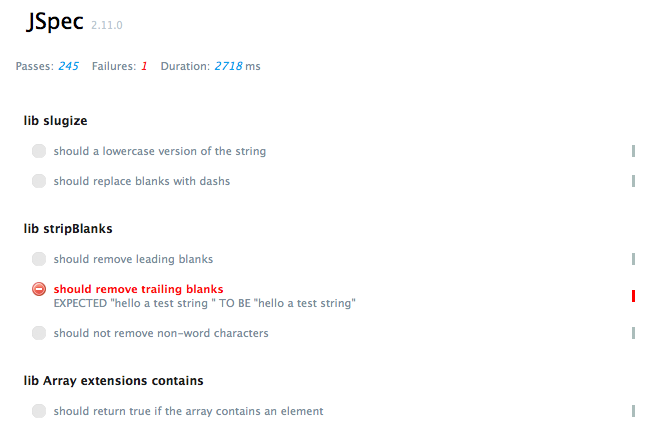
\includegraphics[width=0.9\textwidth]{grafik/jspec-example-bad} 
  \end{center}
  \caption{JSpec: Ein Test schlägt fehl}
  \label{fig:jspec-bad} 
\end{figure}



\subsubsection{Cucumber}
\label{subsec:cucumber}

Bei TDD werden Tests vor dem Programmcode geschrieben, deshalb handelt es sich um Black-Box-Tests \cite{beck:tdd}. Bei diesen ist die Implementierung der zu testenden Programmkomponente nicht bekannt, es wird ausschließlich die zu erwartende Funktionalität bzw. das Ergebnis getestet. Bei Unit Tests ist dies oftmals nicht strikt umsetzbar, da diese sehr feinkörnig Eigenheiten der Komponente testen. Integration Tests dagegen setzen auf einer höheren Ebene an: Hier wird die Funktionalität einer Komponente so beschrieben, dass auch Benutzer ohne technischen Hintergrund die Spezifikation verstehen können. Der Entwicklerin erlaubt dies, vor dem Schreiben des Programmcodes unbelastet von Implementierungsdetails über die Geschäftslogik nachzudenken. 

Auch wenn eine Software-Komponente erfolgreich durch Unit Tests getestet ist, kann die Qualität erst dann als garantiert gelten, wenn die Komponente erfolgreich mit dem Rest der Anwendung integriert ist. Das Testing Framework Cucumber \cite{cucumber:website} bietet ein Grundgerüst, um solche Integration Tests zu erstellen.

Der Test für eine größere zusammengehörende Programmkomponente (z.\,B. Benutzerverwaltung, Benutzung des Gliederungseditors) wird in der \textit{Domain Specific Language (DSL)} von Cucumber ein \textit{Feature} genannt. Jedes Feature spezifiert die Rolle des Benutzers (\textit{As a}), den Inhalt des Features (\textit{I want}) sowie seinen Geschäftswert (\textit{In order to}). Ein Feature enthält mehrere \textit{Stories}, die jeweils die Ausführung einer Software-Funktion von Anfang bis Ende beschreiben (z.\,B. Benutzer-Login, Zeile einrücken). Eine Story enthält die Vorbedingungen (\textit{Given}), die einzelnen Schritte des Benutzers (\textit{When}) und die erwünschten Resultate (\textit{Then}). Ein dem Projekt entnommenes Beispiel findet sich in Listing \ref{lst:cucumber-feature}.

\lstset{language=ruby, style=cucumber}
\medskip
\begin{lstlisting}[caption=Ein Cucumber Feature mit zwei Szenarien,label=lst:cucumber-feature]
Feature: CRUD for outlines
  In order to sort my notes
  As a user
  I want to create, list, update and delete outlines
  
  Scenario: create an outline with note
    When I go to the start page 
      And I follow "New Outline" 
      And I fill in "title" with "Songs"
      And I press "Save"
    Then I should see "Songs"
      And I should see "Here is your new outline"
      And the new note li should be blank
      
  Scenario: edit an outlines title
    Given an outline with the title "Songs"
      And I save
    When I go to the start page
      And I follow "Songs"
      And I follow "Change title or delete this outline"
      And I fill in "title" with "Tunes"
      And I press "Save"
    Then I should see "Title successfully changed"
      When I go to the start page
    Then I should see "Tunes"
      And I should not see "Songs"
\end{lstlisting}

Die Bedeutung der einzelnen Zeilen, \textit{Steps} genannt, muss in weiteren Dateien definiert werden. Jeder Step besteht aus einem Signalwort und einem Regulären Ausdruck, für den ein Block mit Ruby-Code ausgeführt wird. Dabei werden die Resultate der Matching-Gruppen im Regulären Ausdruck dem Block übergeben. Dies ist beispielhaft in Listing \ref{lst:cucumber-steps} demonstriert.


Ein Feature kann auf der Kommandozeile ausgeführt werden (Beispiel in Abbildung \ref{fig:cucumber-bad}). Dabei werden die erfolgreichen Steps grün und die fehlgeschlagenen rot dargestellt, wobei bei letzteren die Fehlermeldungen mit ausgegeben werden.  

\medskip
\begin{lstlisting}[caption=Cucumber Step-Definition,label=lst:cucumber-steps]
Given /^an outline with the title "([^\"]*)"$/ do |title|
  outline = {:kind => 'Outline', :title => title}
  RestClient.put "#{host}/#{database}/#{title}", outline.to_json
end

When /I fill in "(.*)" with "(.*)"/ do |field, value|
  find_by_label_or_id(:text_field, field).set value
end
\end{lstlisting}

\medskip
\begin{figure}[ht] 
  \begin{center}
    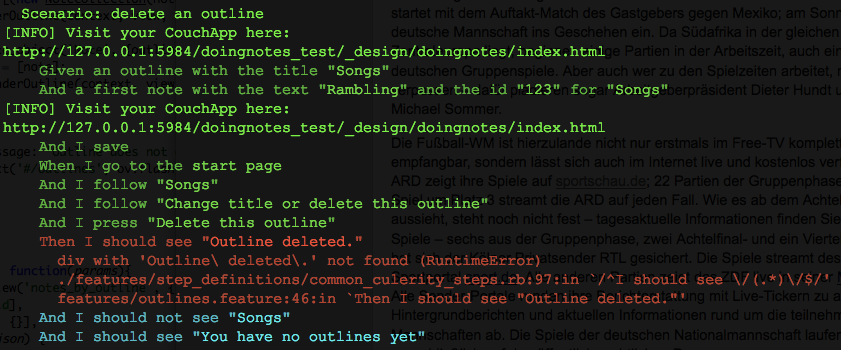
\includegraphics[width=\textwidth]{grafik/cucumber-example-bad} 
  \end{center}
  \caption{Cucumber: Ein Test schlägt fehl}
  \label{fig:cucumber-bad} 
\end{figure}




\subsection{Entwicklungsumgebungen}

\subsubsection{Textmate}

TextMate \cite{textmate:website} ist ein Texteditor für das Betriebssystem Mac OS X. TextMate wurde 2004 von Allan Odgaard herausgegeben. Im August 2006 bekam das Programm den \enquote{Apple Design Award for Best Developer Tool} bei der \enquote{Worldwide Developers Conference} der Firma Apple. TextMate ist ein sehr übersichtlicher Editor \citelit{textmate:latex}. Er hat bei weitem nicht den Funktionsumfang einer Entwicklungsumgebung wie Eclipse oder NetBeans, lässt sich aber durch seine weitreichende Unterstüzung für Skripte und Plugins beliebig erweitern. Für die Bearbeitung der vorliegenden Aufgabe wäre der Einsatz einer solchen integrierten Entwicklungsumgebung nicht zweckmäßig gewesen: Die spezifischen Anforderungen, die die Entwicklung einer Couchapp stellt, werden durch Eclipse zum jetzigen Zeitpunkt nicht erfüllt. 

Textmate bietet Syntax-Highlighting für alle verwendeten Sprachen, Auto-Completion innerhalb einer Datei, projektweite Suche, einfachen Zugriff auf alle Dateien im Projekt, ein übersichtliches Interface mit Tabs für alle geöffneten Dateien. Darüberhinaus ist es leicht, Textmate an besondere Anforderungen anzupassen. So wurde für das Aktualisieren der Designdokumente in der Datenbank ein eigenes Couchapp-Makro entwickelt, was den Entwicklungsprozess beschleunigte.  


\subsubsection{Firefox / Firebug}


In Abschnitt \ref{subsec:nochanges} wird erläutert, warum der Browser Firefox \cite{firefox} in mindestens Version 3.5 als Zielplattform gewählt wurde. Aus diesem Grund wurde die Anwendung mithilfe der Firefox-Erweiterung Firebug \cite{firebug} entwickelt. 

Mit der Firebug können Stylesheets, HTML, das DOM und JavaScript auf einer Webseite untersucht werden. Eine Konsole erlaubt das Loggen von Log-Statements im JavaScript-Code und von HTTP-Requests. Der Quelltext einer Webseite kann ebenfalls live analysiert und auch editiert werden. Dies ermöglicht einfaches Debugging. Es gilt deshalb als besonders beliebt unter Webentwicklern \cite{firebug:beliebt}. Firebug ist das am sechsthäufigsten heruntergeladene Add-on für Firefox \cite{firebug:haeufig}. Es wird von mehr als zwei Millionen Menschen täglich benutzt \cite{firebug:stats}. 

Firebug wurde in diesem Projekt sowohl für Entwicklung des DOMs, für die Gestaltung des Frontends, als auch für einfache Performance-Optimierung des Seitenaufbaus verwendet. 
